% !TeIX spellcheck = cs_CZ
%{\tikzset{external/prefix={tikz/FYZII/}}
% \tikzset{external/figure name/.add={ch09_}{}}
%---------------------------------------------------------------------------------------------------
% file fey2ch09.tex
%---------------------------------------------------------------------------------------------------
%=========================== Kapitola: Elektřina v atmosféře =======================================
\setchaptertoc
\chapter{Elektřina v atmosféře}\label{fyz:IIchapIX}  
  S rozvojem empirické vědy v novověku se ale stále častěji objevovala otázka, co je vlastně
  podstatou blesku. Od poloviny 18. století začali přírodovědci intenzivněji zkoumat elektrické
  jevy. Netrvalo dlouho a v roce 1752 americký polyhistor Benjamin Franklin odvodil na základě svého
  známého experimentu s drakem hypotézu, že atmosférická elektřina opravdu může být zdrojem blesků a
  že jde o mechanismus podobný výbojům statické elektřiny. Následoval vynález bleskosvodu, který
  začal chránit zprvu především věže kostelů, později i lodě na mořích.

  U nás se výzkumu atmosférické elektřiny v téže době věnoval kněz a přírodovědec Prokop Diviš. V
  létě 1754 sestrojil přístroj, fungující jako první dobře uzemněný bleskosvod. Jeho „meteorologický
  stroj“ však měl svou složitou konstrukcí především odvádět atmosférickou elektřinu do země, a tím
  vzniku blesků předcházet, což se nedařilo ani jemu, ani Franklinovi.

  \section{Gradient elektrického potenciálu v atmosféře}\label{fyz:IIchapIXsecI}  
    Za obyčejného dne nad rovinatou pouští nebo nad mořem vzrůstá elektrický potenciál asi o
    \num{100} voltů na metr vzhůru od zemského povrchu. Ve vzduchu tedy existuje vertikální
    elektrické pole \(E\) s velikostí \SI{100}{\V\per\m}. Směr pole je takový, jako kdyby zemský
    povrch měl záporný náboj. To znamená, že venku je potenciál ve výšce nosu o \num{200} voltů
    vyšší než potenciál na úrovni našich chodidel. Mohli bychom se zeptat: „Proč tedy neupevníme ve
    vzduchu ve vzdálenosti jeden metr od sebe dvě elektrody a nevyužijeme těch \num{100} voltů k
    napájení elektrického osvětlení?“ Nebo bychom se mohli podivit: Je-li mezi mým nosem a chodidly
    skutečně napětí 200 voltů, proč když vycházím z budovy, nedostanu elektrický šok?“

    Objasníme nejprve druhou otázku. Naše tělo je poměrně dobrým vodičem. Dotýkáme-li se země, spolu
    s ní vytváříte jednu ekvipotenciální hladinu. Ekvipotenciální hladiny jsou normálně rovnoběžné
    se zemským povrchem (obr. \ref{fyz:fig689a}), ale když je tam naše tělo, poruší se a pole vypadá
    asi tak, jako ukazuje obr. \ref{fyz:fig689b}. Mezi naší hlavou a chodidly je tedy téměř nulové
    napětí. Ze země přechází do naší hlavy náboje a pole se mění.

    \begin{figure}[ht!]
      \centering
      \subcaptionbox{\label{fyz:fig689a}}{\luafigure[0.8]{fyz_fig689a.pdf}}               \newline
      \subcaptionbox{\label{fyz:fig689b}}{\luafigure[0.8]{fyz_fig689b.pdf}}
      \caption{a) rozdělení potenciálu nad zemí. b) rozdělení potenciálu v blízkosti člověka 
               stojícího na otevřeném rovinném prostranství (\cite[s.~748]{Feynman02})}
      \label{fyz:fig689}
    \end{figure}

    Některé z těchto nábojů mohou být neutralizovány ionty ve vzduchu, jejich proud je však velmi
    malý, neboť vzduch je špatným vodičem.

    Jak můžeme měřit takové pole, změní-li se, když do něj něco vložíme? Existuje několik způsobů.
    Jeden způsob je umístit izolovaný vodič do určité vzdálenosti nad zemí a nechat jej tam, dokud
    nebude na stejném potenciálu jako vzduch. Necháme-li jej tam dostatečně dlouho, budou i při malé
    vodivosti vzduchu náboje z (nebo do) vodiče unikat, dokud se jeho potenciál nevyrovná s
    potenciálem vzduchu na stejné úrovni. Pak jej můžeme opět spustit k zemi a změřit změnu
    potenciálu. Rychlejší způsob je použít jako vodič vědro vody s malou dírkou. Vykapávající voda
    odnese přebytečné náboje a vědro bude mít tentýž potenciál jako vzduch. (Jak víme, náboje se
    zdržují na povrchu a odkapáváním kapek se „kousky povrchu“ odlamují.) Potenciál vědra je možné
    změřit elektrometrem.

    \begin{figure}[ht!]
      \centering
      \subcaptionbox{\label{fyz:fig690a}}{\luafigure[0.9]{fyz_fig690a.pdf}}               \newline
      \subcaptionbox{\label{fyz:fig690b}}{\luafigure[0.9]{fyz_fig690b.pdf}}
      \caption{a) Uzemněná kovová deska bude mít stejný plošný náboj jako zemský povrch.
               b) Když se deska přikryje uzemněným vodičem, nebude mít žádný plošný náboj.
               (\cite[s.~707]{Feynman02})}
      \label{fyz:fig690}
    \end{figure}

    Existuje ještě jeden způsob přímého měření \emph{gradientu} potenciálu. Protože existuje
    elektrické pole, má Země svůj povrchový náboj \((σ=\varepsilon_0E)\). Umístíme-li do blízkosti
    zemského povrchu rovnou kovovou desku \(A\) a uzemníme ji, objeví se na ní záporné náboje (obr.
    \ref{fyz:fig690a}). Přikryjeme-li tuto deskujinou uzemněnou vodivou deskou \(B\), objeví se
    náboje na ní a z původní desky \(A\) vymizí. Když odměříme náboj, jenž prochází z desky \(A\) k
    zemi (například galvanometrem připojeným k uzemňovacímu vodiči při jejím zakrývání, můžeme
    zjistit povrchovou hustotu náboje, která na něm byla, a tím zjistit i elektrické pole.

    Když jsme si připomněli, jak je možné elektrické pole v atmosféře měřit, budeme nyní pokračovat
    v jeho popisu. Měření především ukazují, že při výstupu do velkých výšek pole sice existuje, ale
    slábne. Zhruba po padesáti kilometrech je už velmi malé, takže většina změny potenciálu
    (integrál intenzity \(E\)) připadá na menší výšky. Celkový rozdíl potenciálu od povrchu Země k
    horní hranici atmosféry je asi \num{400000} voltů.

  \section{Elektrické proudy v atmosféře}\label{fyz:IIchapIXsecII}   
    Kromě gradientu potenciálu můžeme v atmosféře měřit také proud. Hustota proudu je malá - každým
    metrem čtverečním rovnoběžným se zemským povrchem prochází asi \num{10} pikoampérů. Vzduch
    zřejmě není dokonalý izolant a v důsledku jeho vodivosti prochází od oblohy dolů k zemi malý
    proud, vyvolaný právě popisovaným elektrickým polem.

    \begin{figure}[ht!] %\ref{fyz:fig691}
      \centering
      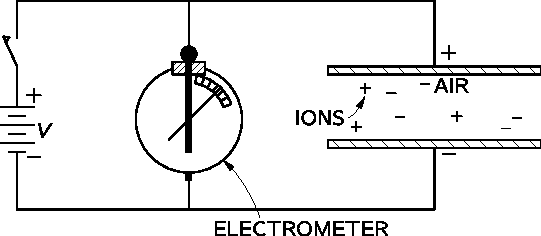
\includegraphics[width=0.8\linewidth]{fyz_fig691.pdf}
      \caption{Měření vodivosti vzduchu způsobené pohybem iontů
               (\cite[s.~707]{Feynman02})}
      \label{fyz:fig691}
    \end{figure}

    Proč je atmosféra vodivá? Mezi molekulami vzduchu se tu a tam vyskytne iont, řekněme molekula
    kyslíku, která přibrala jeden elektron navíc, nebo snad jeden elektron ztratila. Tyto ionty
    nezůstávají osamocené; svým elektrickým polem kolem sebe obvykle shromáždí několik dalších
    molekul. Každý iont se potom stává malou hrudkou, která je spolu s jinými podobnými hrudkami
    unášena polem, a při pomalém pohybu vzhůru nebo dolů vytváří pozorovatelný proud. Odkud ionty
    pocházejí? Nejdříve se lidé domnívali, že vznik iontů způsobuje radioaktivita Země. (Bylo známo,
    že záření z radioaktivních látek ionizuje molekuly ve vzduchu a tím jej dělá vodivým.) Částice,
    například \(\beta\)-záření, vyletují z atomových jader tak rychle, že vytrhávají elektrony z
    atomů a zanechávají za sebou ionty. Z této domněnky ovšem vyplývá, že při výstupu do větších
    výšek bychom našli menší ionizaci, protože všechna radioaktivita se nachází v Zemi - ve
    stopových množstvích radia, uranu, draslíku apod.

    K prověření této teorie vykonali někteří fyzici experiment s balóny ve velké výšce, aby změřili
    ionizaci vzduchu (Hess, r. 1912). Objevili však, že opak je pravdou - ionizace na jednotku
    objemu s výškou roste! (Přístroj byl podobný tomu, který je znázorněn na obr. \ref{fyz:fig691}.
    Dvě desky byly periodicky nabíjeny na napětí \(U\). V důsledku vodivosti vzduchu se desky pomalu
    vybíjely; rychlost vybíjení byla měřena elektrometrem.) Tento nepochopitelný výsledek byl nej
    dramatičtějším objevem v celé historii atmosférické elektřiny.

    Byl vlastně tak dramatický, že podnítil vznik docela nové vědní oblasti - fyziky kosmického
    záření. Problém samotné atmosférické elektřiny zůstal v pozadí. Ionizaci vzduchu způsobovalo
    zřejmě cosi mimozemského; výzkum tohoto zdroje vedl k objevu kosmického záření. Nyní o něm
    nebudeme více hovořit, snad jen tolik, že je zdrojem iontů ve vzduchu. Ačkoli jsou ionty
    neustále odnášeny pryč, produkují částice kosmického záření přicházející z vesmíru neustále nové
    ionty.

    Pro přesnost musíme říci, že kromě iontů vytvořených z molekul, existují i jiné druhy iontů. Ve
    vzduchu se vznášejí droboučké kousky půdy, například velmi jemná prachová zrníčka, a nabíjejí
    se. Nékdy se nazývají \uv{jádra}. Anebo jiný příklad. Při zhroucení mořské vlny se do vzduchu
    vyvrhují malé kapičky. Když se nékterá z nich vypaří, zanechá ve vzduchu vznášející se extrémně
    malý krystalek \ce{NaCl}. Tyto droboučké krystalky mohou potom přibírat náboje a stát se ionty;
    jsou nazývány \uv{velké ionty}.

    \begin{figure}[ht!] %\ref{fyz:fig692}
      \centering
      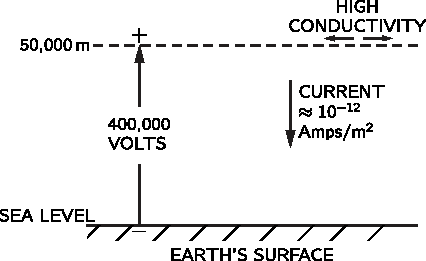
\includegraphics[width=0.9\linewidth]{fyz_fig692.pdf}
      \caption{Typické elektrické poměry za jasného počasí
               (\cite[s.~707]{Feynman02})}
      \label{fyz:fig692}
    \end{figure}

    Malé ionty, tj. ty, které vytvořilo kosmické záření, jsou nejpohyblivější. Protože jsou tak
    malé, pohybují se ve vzduchu rychle - rychlostí asi \SI{1}{\cm\per\s} v poli \SI{100}{\V\per\m}
    neboli \SI{1}{\V\per\cm}. Mnohem větší a hmotnější ionty se pohybují mnohem pomaleji. Ukazuje
    se, že je-li \uv{jader} mnoho, přebírají náboje od malých iontů. Protože \uv{velké ionty} se
    pohybují velmi pomalu, celková vodivost se pak zmenšuje. Vodivost vzduchu je tedy krajně
    proměnlivá, protože je velmi citlivá na množství nečistot v něm. Takových nečistot je mnohem
    více nad souší, kde mohou větry zvedat prach ze země, nebo kde se do vzduchu dostávají
    nejrozmanitější odpadové nečistoty, než nad vodou. Potom nepřekvapuje, že ze dne na den, z
    okamžiku na okamžik, od místa k místu vodivost v blízkosti zemského povrchu ohromně kolísá. V
    každém bodě nad zemským povrchem se značně mění i gradient potenciálu, neboť na různých místech
    přichází dolů z velkých výšek zhruba stejný proud a proměnlivá vodivost při zemském povrchu se
    projeví proměnlivým gradientem potenciálu.

    S výškou rapidně vzrůstá i vodivost vzduchu způsobená driftem iontů, a to ze dvou příčin. 
    Především s výškou vzrůstá ionizace vyvolaná kosmickým zářením. Za druhé, při menší hustotě
    vzduchu se prodlužuje střední volná dráha iontů, které pak mohou mezi srážkami překonat v
    elektrickém poli delší dráhu, což se projeví rapidním vzrůstem vodivosti při výstupu vzhůru.
    Ačkoli je hustota elektrického proudu ve vzduchu pouze několik pikoampérů na metr čtvereční, má
    zemský povrch velmi mnoho takových čtverečních metrů. Celkový elektrický proud, který dosahuje
    zemského povrchu, se téměř nemění a je 1800 ampérů. Tento proud je, samozřejmě, \uv{kladný} - do
    Země přivádí kladné náboje. Máme tedy napětí \num{400 000} voltů při proudu \num{1800} ampérů,
    což představuje výkon \num{700} megawattů.

    Při tak velkém proudu směřujícím dolů by se záporný náboj Země měl brzy neutralizovat. Skutečně
    by na to bylo třeba asi jen půl hodiny. Přesto atmosférické pole existuje, už jen od svého
    objevu, mnohem déle než půl hodiny. Jak se udržuje? Co udržuje elektrické napětí? A mezi čím a
    Zemí? Je tu mnoho otázek. 

    Země je nabitá záporně a potenciál ve vzduchu je kladný. V dostatečně velké výšce je vodivost
    tak velká, že v horizontálním směruje potenciál prakticky stejný. Z aspektu času, o němž zde
    hovoříme, se vzduch ve výšce asi \SI{50}{\km} vlastně stává vodičem. To ještě není výška
    odpovídající tomu, co se nazývá \emph{ionosféra}, v níž vznikají velká množství iontů v důsledku
    fotoelektrických účinků slunečního záření. Ve výšce přibližně \SI{50}{\km} se stává vzduch
    natolik vodivým, že můžeme udělat v naší úvaze o atmosférické elektřině předpoklad, že v této
    výšce existuje prakticky dokonale vodivá plocha, z níž proud vychází dolů. Schéma této situace
    je na obr. \ref{fyz:fig692}. Otázkou je, jak je tam udržován kladný náboj. Jak se dostává zpět?
    Protože přitéká-li dolů k zemi, musí být potom nějak přečerpáván zpět nahoru. To byla dost
    dlouho jedna z největších záhad atmosférické elektřiny.

    \begin{figure}[ht!] %\ref{fyz:fig693}
      \centering
      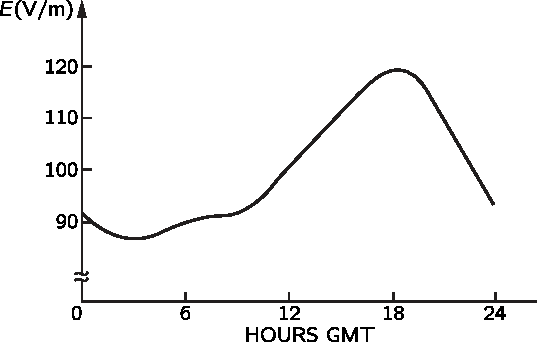
\includegraphics[width=0.9\linewidth]{fyz_fig693.pdf}
      \caption{Střední denní variace gradientu potenciálu v atmosféře za jasného dne nad oceány;
               údaje se vztahuji ke greenwichskému času. (\cite[s.~707]{Feynman02})}
      \label{fyz:fig693}
    \end{figure}

    Jakákoliv informace, kterou dokážeme získat, by mohla poskytnout klíč k této záhadě, nebo
    alespoň o ní něco říct. Je tu jeden zajímavý úkaz: Měříme-li proud (který je stabilnější
    veličinou než gradient potenciálu) například nad mořem nebo v kontrolovaných podmínkách a velmi
    pečlivě vypočteme průměry, abychom se zbavili náhodných hodnot, zjistíme, že existuje jeho denní
    variace. Průměr získaný z mnoha měření nad oceány závisí na čase zhruba tak, jak ukazuje obr.
    9.5Proudse mění asi o \SI{\pm15}{\percent} a maxima dosahuje v sedm večer londýnského času.
    Překvapující na celé věci je, že nezáleží na tom, kde se proud měří - v Atlantiku, Tichém
    oceánu, nebo v Severním ledovém oceánu - největší hodnoty dosahuje tehdy, když je v Londýně sedm
    večer. Na celém světě je proud v maximu v \SI{7.00}{\hour} večer londýnského času a v minimu ve
    \SI{4.00}{\hour} ráno londýnského času.

    Jinými slovy, závisí na absolutním zemském čase, a ne na lokálním čase v místě měření. V jednom
    ohledu to není tak záhadné; shoduje se to s naší představou, že nahoře existuje velká
    horizontální vodivost, která znemožňuje, aby se napětí mezi zemí a vrchní vrstvou atmosféry
    měnilo podle místa. Jakékoliv změny potenciálu by měly být celosvětové, a také jsou. Od této
    víme, že napětí horní vrstvy atmosféry klesá a stoupá o \SI{15}{\percent} v závislosti na
    absolutním čase na zemi.
  
  \section{Původ atmosférických proudu}\label{fyz:IIchapIXsecIII} 
  
    Dále se budeme zabývat zdrojem velkých záporných proudů, které musí téci „shora“ k zemskému
    povrchu, aby udržely záporný náboj Země. Kde je tento zdroj? Zdroj ukazuje obr.
    \ref{fyz:fig694}. Je to bouřka a bouřkový blesk. Ukazuje se, že blesky „nevybíjejí“ to napětí, o
    kterém jsme hovořili (jak by se vám mohlo zprvu zdát). Bouřky s blesky přivádějí do země záporné
    náboje. Když udeří blesk, s pravděpodobností 10 : 1 dolů přináší velké množství záporného
    náboje. Jsou to právě bouřky na celém světě, které nabíjejí Zemi elektrickým proudem s průměrem
    \SI{1800}{\A}, jenž se potom vybíjí v oblastech s klidným počasím.

    \begin{figure}[ht!] %\ref{fyz:fig694}
      \centering
      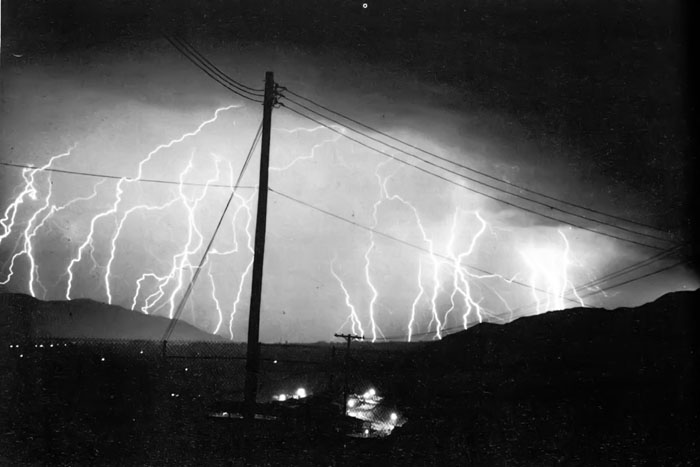
\includegraphics[width=1\linewidth]{fyz_fig694.jpg}
      \caption{Mechanizmus generující elektrické pole v atmosféře (foto William L. Widmayer)
              (\cite[s.~707]{Feynman02})}
      \label{fyz:fig694}
    \end{figure}

    Na celé zeměkouli je asi \num{40 000} bouřek za den. Bouřky můžeme pokládat za „zdroje“, které
    načerpávají elektřinu do horních vrstev atmosféry a udržují rozdíl potenciálů. Nyní si
    představte, jak vypadá naše Země - odpoledne jsou bouřky v Brazílii, tropické bouřky v Africe
    atd. Vědci odhadli počet blesků, které v každém okamžiku zasahují zeměkouli, a není snad třeba
    dodávat, že jejich odhady více či méně souhlasí s měřeními napětí. Na celé zeměkouli je největší
    bouřková aktivita asi v sedm hodin večer londýnského času. Ale dělat takové odhady bouřek je
    velmi těžké a udělaly se pouze potom, když se vědělo, jaká variace se má v nich objevit.
  
    Problém je totiž v tom, že nemáme dostatek pozorování na moři a ve všech částech světa, abychom
    počet bouřek znali přesně. Ti vědci, kteří se domnívají, že „to udělali správně“, přicházejí k
    výsledku, že na celém světě udeří asi \num{100} blesků za sekundu s maximem bouřkové aktivity v
    7.00 h večer greenwichského středního času.

    Abychom porozuměli, jak pracují tyto zdroje, všimneme si bouřky detailněji. Co se děje uvnitř
    bouřky? Popíšeme to, co zatím známe. Vnikáme-li do tohoto neobyčejného úkazu v reálné přírodě,
    místo dokonale vodivých koulí uvnitř jiných koulí, jež umíme tak pěkně řešit, zjišťujeme, že
    toho nevíme příliš mnoho. A je to opravdu vzrušující. Každý, kdo zažil bouřku, se z ní radoval,
    nebo byl vystrašený, nebo alespoň něco pociťoval. A na těch místech v přírodě, které evokují
    emoce, obvykle nacházíme i odpovídající složitost i tajemnost přírody. Není možné exaktně
    popsat, jak se bouřka odehrává, neboť ještě mnoho nevíme. Ale zkusíme trochu pohovořit o tom, co
    se při ní děje.

    \begin{figure}[ht!] %\ref{fyz:fig938}
      \centering
      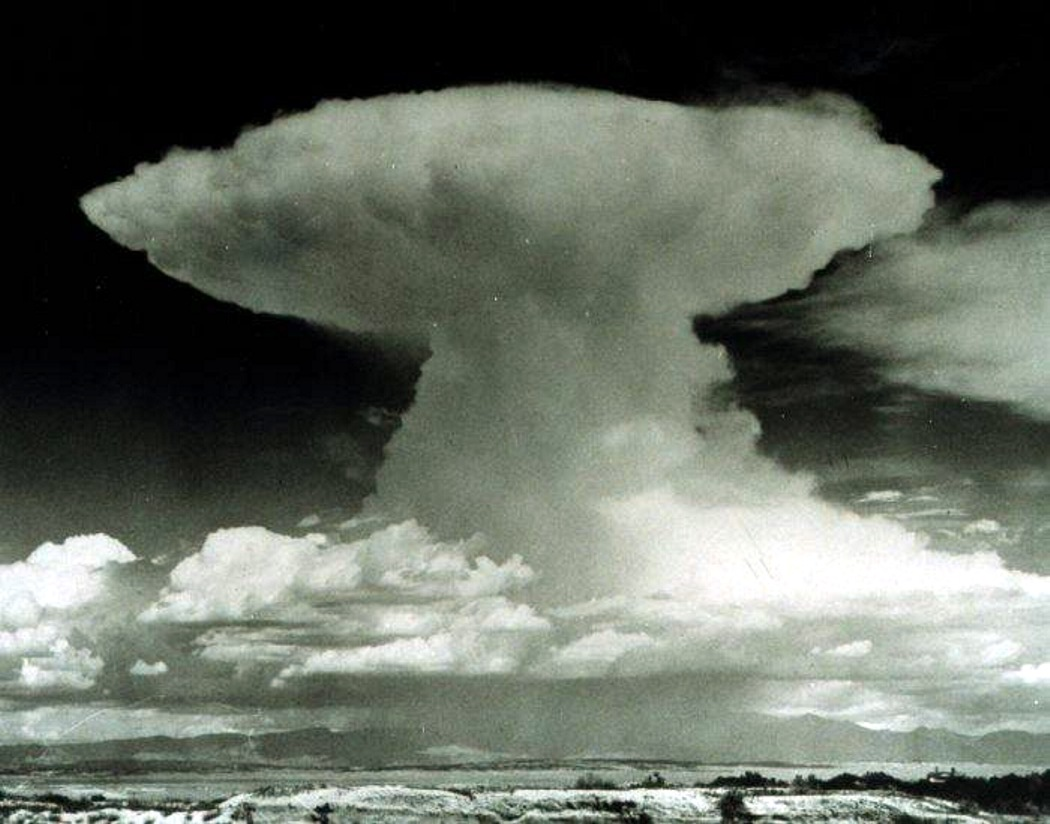
\includegraphics[width=1\linewidth]{fyz_fig938.png}
      \caption{Bouřkový oblak neboli Cumulonimbus je nejčastějším zdrojem blesků. Zdroj: NOAA.}
      \label{fyz:fig938}
    \end{figure}

    % https://www.zonerama.com/brahe/Album/5118608
    \begin{figure}[ht!] %\ref{fyz:fig694}
      \centering
      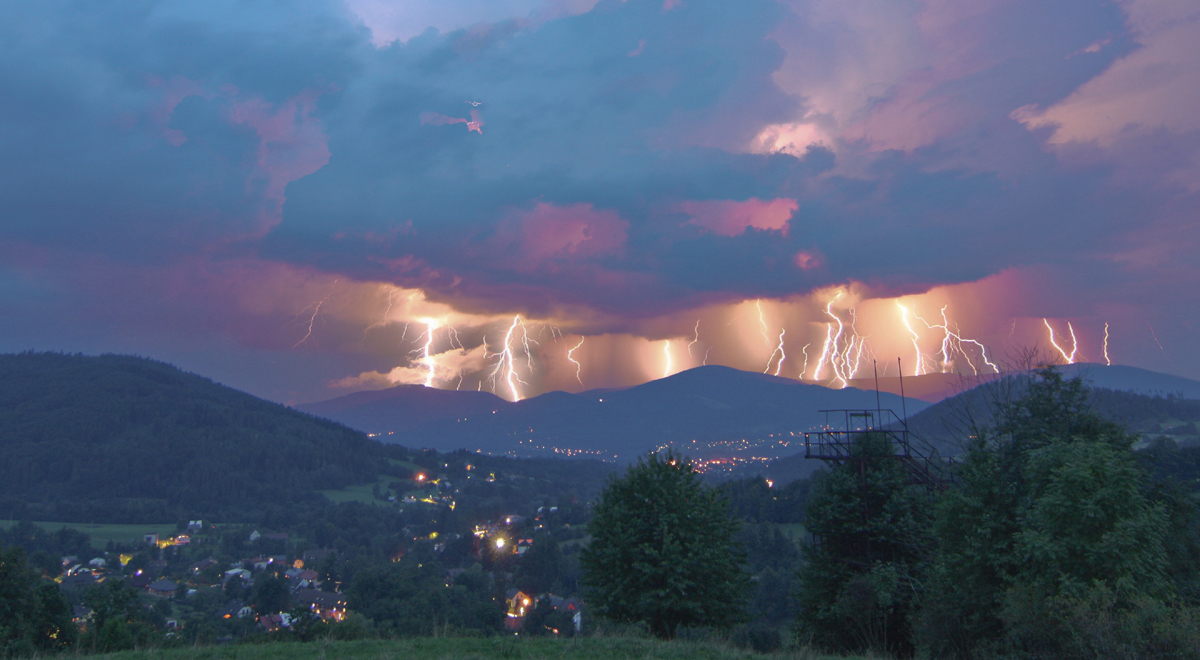
\includegraphics[width=1\linewidth]{fyz_fig694a.jpg}
      \caption{Bouřka na Beskydy. Foto: Martin Popek}
      \label{fyz:fig694a}
    \end{figure}

  \section{Bouřky}\label{fyz:IIchapIXsecIV}   
    S bouřkami se v běžném životě setkáváme pravidelně, a snad právě proto většina z nás nabyla
    dojmu, že jde o dobře prozkoumaný komplex jevů. Opak je ale pravdou. Nejasnosti jsou nejen kolem
    detailů nabíjení bouřkových oblaků, ale není ani známé, proč dojde k samotnému průrazu a vzniku
    blesku. Z meteorologického hlediska představuje bouřka nejvýraznější projev konvekce v
    atmosféře. Podmínky vzniku bouřky jsou:
    \begin{itemize}[noitemsep]
      \item instabilní zvrstvení vzduchové hmoty do vysokých hladin atmosféry,
      \item vysoká relativní vlhkost při zemi i ve výšce,
      \item přítomnost vnější síly, která iniciuje vertikální pohyb.
    \end{itemize}
    Základním stavebním kamenem všech bouřek je bouřková (neboli konvekční) buňka. Tato buňka
    prochází jednotlivým stádii vývoje uvnitř oblaku typu \textbf{cumulunimbus - Cb}. Comulunimbus
    je zpravidla komplexem několika buňek, které postupně vznikají, procházejí jednotlivými stádii
    a pak zanikají. 

    Každá buňka představuje ohraničenou oblast v horizontálním směru, v níž probíhají všechny
    základní procesy. Obvykle vedle sebe existuje několik buněk, z nichž v každé probíhá zhruba
    totéž, ale ne současně (obr. \ref{fyz:fig689b}). 

    \begin{figure}[ht!]
      \centering
      \subcaptionbox{\label{fyz:fig937a}}{\luafigure[0.45]{fyz_fig937a.png}}\hspace{1em} 
      \subcaptionbox{\label{fyz:fig937b}}{\luafigure[0.45]{fyz_fig937b.png}}
      \caption{a) Ve všech hladinách zasažených tvořící se bouřkovou buňkou se projevuje
      konvergence proudění – okolní vzduch ze všech stran vtéká do prostoru vzestupného proudu. b)
      Vznikající Cb je tvořen oddělenými buňkami v různých fázích vývoje. Ve většině případů se v
      oblaku nachází několik vzestupných i sestupných proudů najednou. Vznikají nové buňky a každá
      nová roste do větší výšky než buňka předchozí, přičemž staré zanikají.}
      \label{fyz:fig937}
    \end{figure}
    
    Obr. \ref{fyz:fig695} schematicky naznačuje, jak taková \emph{buňka} vypadá v počátečním
    stádiu bouřky. Ukazuje se, že v určitém místě ve vzduchu za určitých podmínek, které popíšeme
    dále, dochází k obecnému vzestupu vzduchu rychlostí, která směrem vzhůru roste. Dole teplý a
    vlhký vzduch se při vzestupu ochlazuje a vláha tam kondenzuje. Na obrázku označují hvězdičky
    sníh a kroužky déšť. Protože je však stoupající proud dost velký a kapky jsou dost malé, ani
    sníh ani déšť v tomto stádiu nedopadnou dolů. To je počáteční stádium a ještě ne opravdová
    bouřka v tom smyslu, že při zemi se nic neděje. Současně, jak teplý vzduch stoupá, dochází k
    přívalu vzduchu ze stran; to je důležitý fakt, jenž se po mnoho let zanedbával. Vzduch tedy
    stoupá nejen zdola, ale i určité množství vzduchu ze stran.    

    \begin{figure}[ht!] %\ref{fyz:fig695}
      \centering
      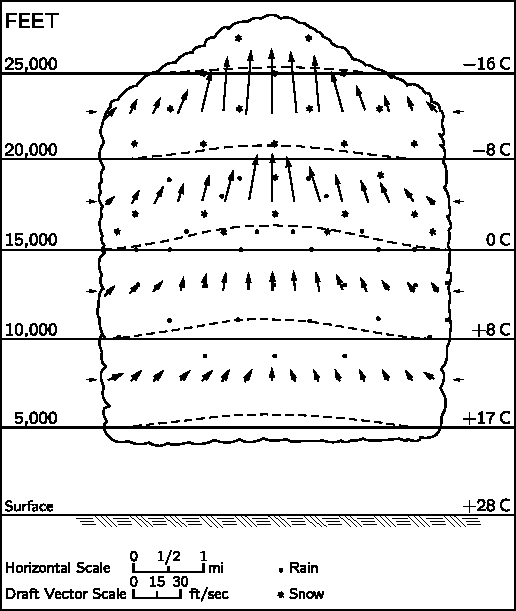
\includegraphics[width=0.9\linewidth]{fyz_fig695.pdf}
      \caption{Bouřková buňka v prvních stádiích vývoje (\cite[s.~707]{Feynman02})}
      \label{fyz:fig695}
    \end{figure}

    Proč vzduch takto stoupá? Jak víme, nahoře je vzduch chladnější. Slunce vyhřívá zemský povrch
    a vysoko v atmosféře vyzařuje vodní pára teplo vzhůru; proto je ve velkých výškách vzduch
    chladný, velmi chladný, zatímco níže je vzduch teplý. Můžeme říci: „Pak je to velmi
    jednoduché. Teplý vzduch je lehčí než chladný, proto je tato kombinace mechanicky nestabilní a
    teplý vzduch stoupá.“ Samozřejmě, je-li v různých výškách různá teplota, vzduch je
    termodynamicky nestabilní. Kdyby byl ponechán sám o sobě, získal by všechen vzduch tutéž
    teplotu. Ale vzduch není ponechán sám o sobě, neboť Slunce vždy svítí (ve dne). Ve skutečnosti
    tedy nejde o problém termodynamické ale mechanické rovnováhy. Nakreslíme-li graf (obr.
    \ref{fyz:fig696}) závislosti teploty vzduchu na výšce nad zemským povrchem, za obvyklých
    podmínek bychom dostali klesající křivku označenou a při nárůstu výšky teplota klesá.

    \begin{figure}[ht!] %\ref{fyz:fig696}
      \centering
      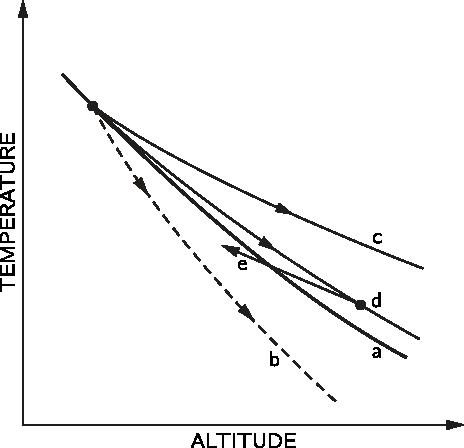
\includegraphics[width=0.9\linewidth]{fyz_fig696.pdf}
      \caption{Závislost teploty atmosféry na výšce; a) - statická atmosféra; b) - adiabatické
              ochlazování suchého vzduchu, c) - adiabatické ochlazování vlhkého vzduchu, d) -
              vlhký vzduch s určitou příměsí okolního vzduchu (\cite[s.~707]{Feynman02})}
      \label{fyz:fig696}
    \end{figure}

    Jak může být atmosféra stabilní? Proč horký vzduch zdola prostě nevystoupí nahoru k chladnému?
    Kdyby vzduch stoupal, jeho tlak by klesal a - máme-li namysli určitý balík stoupajícího
    vzduchu - adiabaticky by se rozpínal. (Teplo by do něj nepřicházelo a ani neunikalo, neboť v
    takových velkých rozměrech, o jakých uvažujeme, není dost času na přechod velkého množství
    tepla.) Náš balík by se tedy při stoupání ochlazoval. Závislost teploty na výšce při takovém
    adiabatickém procesu znázorňuje křivka \emph{b} na obr. \ref{fyz:fig696}. Jakýkoliv vzduch,
    který se nahoru dostal zdola, by byl \emph{chladnější} než prostředí, do kterého vnikl. Takže
    horký vzduch nemá důvod stoupat; kdyby stoupal, ochlazoval by se na nižší teplotu než má
    vzduch, který už tam je, stával by se těžším než okolní vzduch, zachtělo by se mu opět dolů.
    Za pěkného, jasného dne s velmi malou vlhkostí existuje určitý pokles teploty v atmosféře s
    výškou. Obecně je menší než maximální stabilní spád, který reprezentuje křivka \emph{b}.
    Vzduch se tehdy nachází ve stavu stabilní mechanické rovnováhy.

    Na druhou stranu, uvažujeme-li o balíku vzduchu, který obsahuje mnoho vodní páry a stoupá
    vzhůru, bude křivka jeho adiabatického ochlazování jiná. Při jeho rozpínání a ochlazování se v
    něm obsažená vodní pára bude kondenzovat a kondenzující voda bude uvolňovat teplo. Vlhký
    vzduch proto není ochlazován tak intenzivně jako suchý. Začne-li tedy stoupat vzduch, který má
    nadprůměrnou vlhkost, bude se jeho teplota měnit podle křivky \emph{c} na obr.
    \ref{fyz:fig696}. Trochu se ochladí, ale ještě stále bude teplejší než okolní vzduch v téže
    výšce. Máme-li tedy oblast teplého, vlhkého vzduchu a něco ji přiměje stoupat, vždy zůstane
    lehčí a teplejší než vzduch okolo a bude pokračovat ve stoupání až do obrovských výšek. V tom
    spočívá podstata mechanismu, jenž přivádí vzduch v bouřkové buňce k výstupu.

    Tak jednoduše se bouřková buňka vysvětlovala dlouhé roky. Pozdější měření však ukázala, že
    teplota v oblaku v různých výškách nebyla ani přibližně tak vysoká, jak by vyplývalo z křivky
    \emph{c}. Příčina je v tom, že když „bublina“ vlhkého vzduchu stoupá, unáší s sebou vzduch z
    okolí a je jím ochlazována. Graf závislosti teploty na výšce vypadá tak, jako křivka \emph{d},
    která je mnohem blíže k původní křivce než ke křivce \emph{c}.

    \begin{figure}[ht!] %\ref{fyz:fig697}
      \centering
      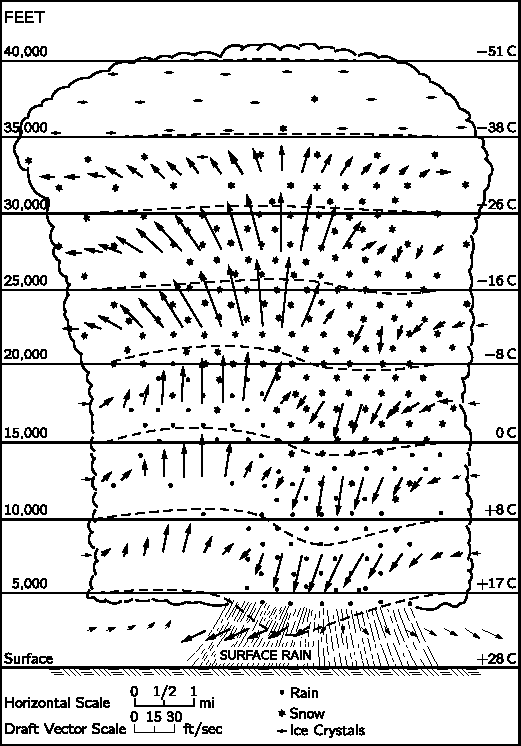
\includegraphics[width=0.9\linewidth]{fyz_fig697.pdf}
      \caption{Zralá bouřková buňka (\cite[s.~707]{Feynman02})}
      \label{fyz:fig697}
    \end{figure}

    Poté, co začala právě popsaná konvekce, vypadá svislý průřez bouřkové buňky tak, jak ukazuje
    obr. \ref{fyz:fig697}. Jde o tzv. „zralou“ bouřku. V ní vzniká velmi rychlé vzestupné
    proudění, jež v tomto stádiu sahá asi až do \SIrange{10}{15}{\km} a někdy i mnohem výše.
    Bouřková oblaka s probíhající kondenzací vystupují z celkového řetězu oblaků, unáší je
    vzestupný proud rychlostí přibližně \SI{100}{\km\per\hour}. Když je vodní pára unášena vzhůru
    a kondenzuje, tvoří drobné kapičky, které se rychle ochlazují na teploty pod bodem mrazu. Měly
    by zmrznout, ale nemrznou hned - jsou „přechlazené“. Voda a jiné kapaliny se obvykle před
    krystalizací snadno ochladí pod své teploty tuhnutí, neobsahují-li jádra“, na nichž by
    krystalizační proces začal. Vodní kapka zmrzne na malý kousek ledu, pouze obsahuje-li nějaký
    kousíček materiálu - takový, jako droboučký krystalek NaCl. V rovnováze se potom vodní kapky
    vypařují a ledové krystaly rostou. Tak voda v určitém okamžiku rychle mizí a stejně rychle se
    tvoří led. Kromě toho může docházet k přímým srážkám vodních kapek s ledem - jejich důsledkem
    je, že přechlazená voda se přichytává ke krystalkům ledu a okamžitě krystalizuje. V určitém
    stádiu rozpínání oblaku tedy dochází k prudkému hromadění velkých částic ledu.

    Jsou-li částice ledu dost těžké, začnou propadat stoupajícím proudem vzduchu, který je už
    nemůže udržet. Při pádu s sebou unášejí trochu vzduchu a začíná sestupný proud. A je dost
    překvapující, o čemž je snadné se přesvědčit, že jakmile sestupný proud začal, udržuje se sám
    do sebe. Vzduch se nyní sám žene dolů.

    \begin{figure}[ht!] %\ref{fyz:fig698}
      \centering
      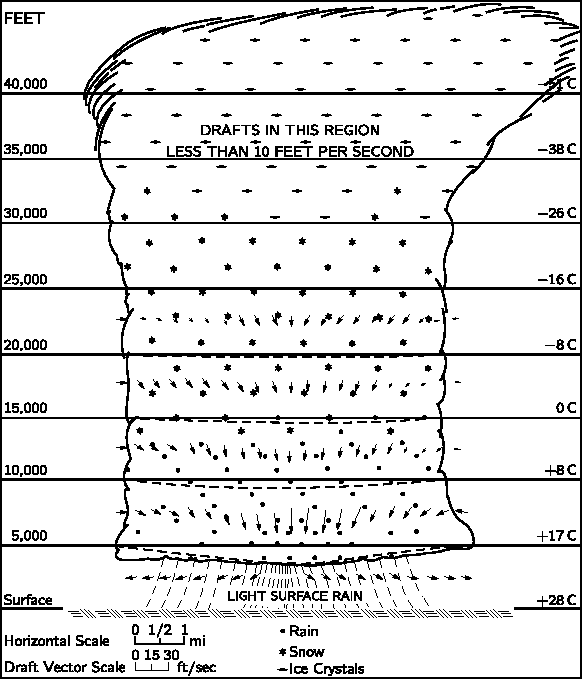
\includegraphics[width=0.9\linewidth]{fyz_fig698.pdf}
      \caption{Cumulonimbus (Cb) je vrcholná fáze konvekce v atmosféře. Dříve uvedené procesy nyní
              dosahují svých maxim. Oblak je velice mohutný a hustý s velkým vertikálním rozsahem
              a má obvykle tvar ohromných kup nebo věží. (\cite[s.~707]{Feynman02})}
      \label{fyz:fig698}
    \end{figure}

    Všimněte si, že křivka \emph{d} na obr. \ref{fyz:fig696} má pro reálné rozdělení teploty v
    oblaku jiný sklon než křivka \emph{c} platící pro vlhký vzduch. Teplota padajícího vlhkého
    vzduchu se bude měnit tak, jak udává sklon křivky \emph{c} a bude tedy při dostatečně velkém
    poklesu nižší než teplota okolí, což na obrázku vyznačuje křivka \emph{e}. V té chvíli však
    bude padající vzduch mít větší hustotu než okolní prostředí a bude pokračovat v rychlém
    sestupu. Můžeme namítnout: „To je věčný pohyb. Nejdříve dokazujeme, že vzduch musí stoupat, a
    když jej máme nahoře, s velkou vervou dokazujeme, že musí padat“ Ale nejde o věčný pohyb. V
    nestabilních podmínkách, kdy je teplý vzduch hnán vzhůru, musí samozřejmě něco přijít na jeho
    místo. Taktéž je pravda, že klesající chladný vzduch by ihned zaujal místo teplého vzduchu,
    ale uvědomme si, že to, co přichází dolů, není původní vzduch. První teorie o izolovaném,
    nejdříve stoupajícím a vzápětí klesajícím oblaku měly určitý háček: potřebovaly déšť k udržení
    sestupného proudu. Tomuto důvodu lze těžko uvěřit. Jakmile si uvědomíme, že k stoupajícímu
    vzduchu je přimíšeno dost vzduchu, který se v uvažované výšce nacházel původně, termodynamické
    důvody vás donutí uznat, že může docházet k poklesu chladného vzduchu, který se původně
    nacházel v nějaké velké výšce. To objasňuje obraz aktivní bouřky, schematicky nakreslený na
    obr. \ref{fyz:fig697}.

    Jakmile se vzduch dostane dolů, začne ze spodní části bouřkového mraku pršet. Kromě toho se
    poměrně chladný vzduch šíří po dosažení zemského povrchu na všechny strany. Proto je
    bezprostředně před deštěm pozorován chladný vítr, varující nás před bouřkou. V bouřce samotné
    se objevují náhlé a nepravidelné poryvy větru, v oblaku vzniká ohromná turbulence. Ale v
    podstatě jde o vzestupný a potom sestupný proud - obecně velmi komplikovaný proces.

    Okamžik, kdy začíná pršet, je okamžikem, kdy začíná velké sestupné proudění a je i okamžikem,
    kdy vlastně vznikají elektrické úkazy.

    Dříve než popíšeme blesk, však chceme zakončit naše vyprávění tím, že se podíváme, co se s
    bouřkovou buňkou stane asi po půl hodině nebo po hodině. Buňka vypadá tak, jak ukazuje obr.
    \ref{fyz:fig698}. Vzestupný proud ustane, protože už není dost teplého vzduchu k jeho udržení.
    Nějaký čas ještě prší, poslední velké kapky dopadají dolů a vše se postupně uklidňuje, ačkoliv
    ve vzduchu ještě zůstaly malé krystalky ledu. Protože ve velké výšce dují větry v různých
    směrech, rozptyluje se horní část oblaku obvykle do tvaru kovadliny. Buňka končí svůj život.
  
  \section{Mechanismus oddělování nábojů}\label{fyz:IIchapIXsecV} 
    Nyní chceme popsat z hlediska našich cílů nejdůležitější aspekt - vznik elektrických nábojů.
    Nejrůznější experimenty, včetně letadel prolétajících bouřkami (piloti, kteří to dělají, jsou
    stateční lidé!), ukazují, že rozdělení náboje v bouřkové buňce vypadá nějak tak, jak je
    nakresleno na obr. \ref{fyz:fig699}. Vrchol buňky je nabit kladně a spodek záporně - s výjimkou
    malé lokální oblasti kladného náboje na dně oblaku, která způsobuje dost starostí. Nezdá se, že
    by někdo věděl, proč existuje a jaký má význam - zda je sekundárním efektem kladného padajícího
    deště nebo podstatnou částí celého mechanismu. Situace by se hodně zjednodušila, kdyby tato
    mladá oblast neexistovala.

    V každém případě převážně záporný náboj dole a kladný náboj nahoře představuje správnou polaritu
    zdroje, který by měl nabíjet Zemi záporně. Kladné náboje jsou ve výšce \SIrange{6}{7}{\km}, kde
    je teplota vzduchu asi \SI{-20}{\degreeCelsius}, zatímco záporné náboje jsou ve výšce
    \SIrange{3}{4}{\km} při teplotách mezi \SIrange{0}{-10}{\degreeCelsius}.

    \begin{figure}[ht!] %\ref{fyz:fig699}
      \centering
      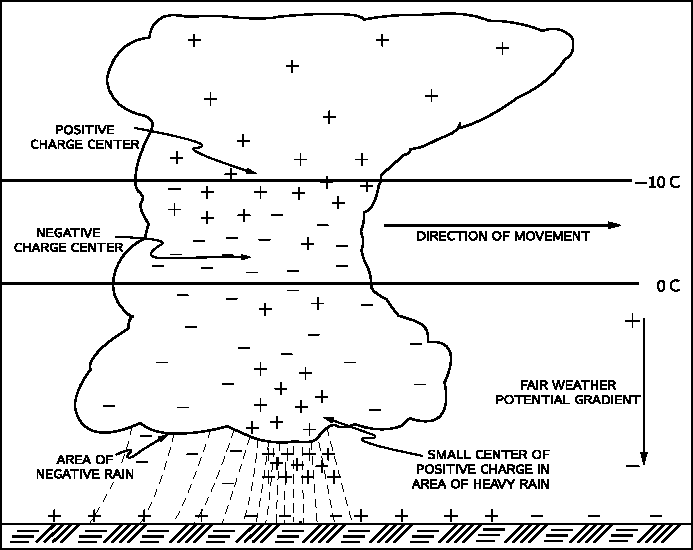
\includegraphics[width=1\linewidth]{fyz_fig699.pdf}
      \caption{Rozdělení elektrických nábojů ve zralé bouřkové buňce (\cite[s.~707]{Feynman02})}
      \label{fyz:fig699}
    \end{figure}

    Náboj vespod oblaku je dostatečně velký, aby vytvořil mezi oblakem a Zemí napětí 20 nebo 30, ba
    i 100 milionů voltů, což je mnohem více než 0,4 milionu voltů mezi „oblohou“ a zemským povrchem
    při jasném počasí. Tato velká napětí způsobují průrazy vzduchu a vyrážejí obrovské obloukové
    výboje. Při průrazu přecházejí záporné náboje zespod oblaku do země ve formě úderů blesku.

    Nyní si blíže všimneme charakteru blesku. Především v okolí existují tak velká napětí, že
    dochází k průrazu vzduchu. Blesky mohou udeřit mezi různými částmi téhož oblaku, mezi různými
    oblaky nebo mezi oblakem a Zemí. V každém nezávislém výbojovém záblesku, v úderu blesku, který
    vidíte, se dolů přenáší náboj přibližně 20 až 30 coulombů. Otázkou je, kolik je třeba času, aby
    oblak generoval těch 20 až 30 coulombů, jež odnesl blesk? Je to možné určit měřením - daleko od
    oblaku - elektrického pole vytvořeného dipólovým momentem oblaku. V takových měřeních se
    zjišťuje náhlý pokles pole při úderu blesku a následující exponenciální návrat do původní
    velikosti s časovou konstantou, která případ od případu trochu kolísá kolem pěti sekund. Oblaku
    tedy stačí pouze 5 sekund po každém úderu blesku, aby znovu vytvořil svůj náboj. To však nutně
    neznamená, že přesně každých 5 sekund následuje další úder blesku, protože se mění geometrie
    situace apod. Údery se dostavují více méně nepravidelně, ale je důležité, že znovu vytvoření
    původních podmínek zabere asi 5 sekund. V bouřkovém generátoru tedy procházejí proudy přibližně
    4 ampéry. To znamená, že každý model, který má vysvětlit, jak bouřka generuje elektřinu, musí
    být modelem s dostatkem „šťávy“ - musí to být obrovské, rychle pracující zařízení.

    Dříve než se dostaneme dále, všimněme si něčeho, co je skoro určitě docela bezvýznamné, ale
    přesto zajímavé, neboť ukazuje vliv elektrického pole na vodní kapky. Řekli jsme, že to nemusí
    mít význam, neboť jde pouze o pokus, který je možné provést v laboratoři s proudem vody, aby se
    demonstroval značný účinek elektrického pole na vodní kapky. V bouřce nejde o proud vody, tam je
    oblak kondenzujícího ledu a vodních kapek. Proto otázka mechanismu uplatňujícího se v bouřce
    pravděpodobně nijak nesouvisí s tím, co můžete vidět na jednoduchém pokusu, který popíšeme.
    Připojíme-li k vodovodnímu kohoutku nástavec se zúženým hrdlem a nasměrujeme ho přímo vzhůru
    (obr.\ref{fyz:fig700}), bude voda vystupovat tenkým proudem, jenž se případně rozpráší na malé
    kapičky. Vytvoříme-li v prostoru vodního proudu u nástavce elektrické pole (například pomocí
    nabité tyčinky), tvar proudu se změní. Zjistíte, že při slabém elektrickém polije proud
    rozdroben na menší počet velkých kapek. Použijete-li však silnější pole, rozpráší se proud na
    velké množství drobounkých kapiček, menších než předtím\footnote{Praktický způsob pozorování
    rozměrů kapek je nechat proud dopadat na velkou kovovou desku. Větší kapky způsobují silnější
    šum.}. Při slabém elektrickém poli se uplatňuje tendence zabránit rozbití proudu na kapky. Při
    silnějším poli však tendence rozdělit proud do kapek roste.

    \begin{figure}[ht!] %\ref{fyz:fig700}
      \centering
      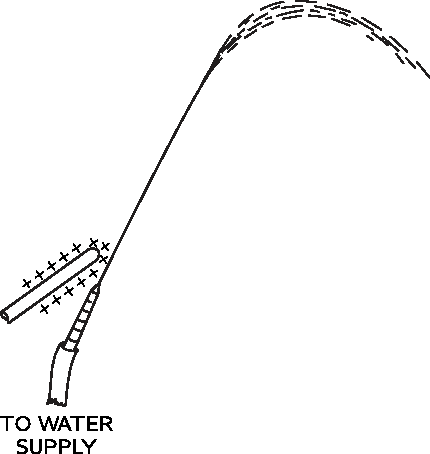
\includegraphics[width=0.8\linewidth]{fyz_fig700.pdf}
      \caption{Proud vody s elektrickým polem v blízkosti nástavce (\cite[s.~707]{Feynman02})}
      \label{fyz:fig700}
    \end{figure}

    Tyto úkazy je možné vysvětlit takto. Vytéká-li z nástavce proud vody a prochází slabým
    elektrickým polem, nabije se jedna strana vodního proudu trochu kladně a druhá strana trochu
    záporně. Budou se navzájem přitahovat a jevit větší tendenci splynout, než jevily předtím -
    proud se bude méně rozprašovat. Na druhé straně, je-li pole silnější, bude náboj každé
    jednotlivé kapky mnohem větší a sám náboj bude svým vlastním odpuzováním napomáhat rozdrobování
    kapek. Každá kapka se rozbije na mnoho menších, z nichž každá bude nabita, takže se budou
    všechny navzájem odpuzovat a rychle se rozptýlí. Zvětšujeme-li tedy pole, rozptýlí se v něm
    vodní proud jemněji. Jediné, na co tu chceme poukázat, je to, že za určitých podmínek může
    elektrické pole mít na kapky velký vliv. Přesný mechanismus toho, co se děje v bouřce, není
    vůbec známý a vůbec není nutné klást ho do souvislosti s tím, co jsme právě popsali. Zahrnuli
    jsme to sem pouze proto, abychom získali představu o složitosti jevů, které by tu mohly hrát
    úlohu. Ve skutečnosti nikdo nevytvořil teorii oblaků založenou na této představě.

    Rádi bychom popsali dvě teorie, jež byly vymyšleny, aby se vysvětlilo rozdělení náboje v bouřce.
    Všechny teorie obsahují myšlenku, že částice v dešťových srážkách mají určitý náboj a vzduch má
    náboj opačný. K rozdělení elektrického náboje pak dochází pohybem srážkových částic - vody nebo
    ledu - ve vzduchu. Jediná otázka je: Jak se kapky nabíjejí? Jedna ze starších teorií se nazývá
    teorie „trhání kapky“. Kdosi objevil, že roztrhne-li se vodní kapka proudem vzduchu na dvě
    části, nabije se voda kladně a vzduch záporně. Tato teorie má několik nedostatků, z nichž
    nejvážnější je ten, že dává nesprávné znaménko. Kromě toho v převážné většině bouřek v mírném
    pásu provázených blesky bývají srážky ve velkých výškách nikoliv vodní, ale ledové.

    Z toho co jsme právě řekli, je vidět, že kdybychom si dokázali nějak představit, jak může kapka
    nabýt shora a zespodu opačné náboje, a kdybychom také znali nějaký důvod, proč se ve vzdušném
    proudu s velkou rychlostí kapky trhají na nestejné části (větší vpředu a menší vzadu v důsledku
    pohybu vzduchu nebo něčeho jiného), měli bychom teorii (odlišnou od dosud známých!). V důsledku
    odporu prostředí by pak malé kapky nepadaly ve vzduchu tak rychle jako velké a došlo by k
    oddělení opačných nábojů. Jak vidíme, je možné vymýšlet si nejrozmanitější možnosti.


    \begin{figure}[ht!] %\ref{fyz:fig701}
      \centering
      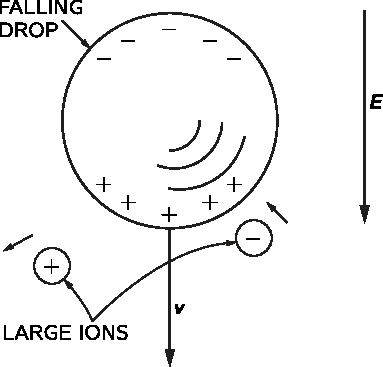
\includegraphics[width=0.7\linewidth]{fyz_fig701.pdf}
      \caption{Teorie C. T. R. Wilsona o oddělování nábojů v bouřkovém oblaku
               (\cite[s.~707]{Feynman02})}
      \label{fyz:fig701}
    \end{figure}

    Jedna z důvtipnějších a v mnoha směrech uspokojivějších teorií než teorie trhajících se kapek je
    teorie C. T. R. Wilsona. Popíšeme ji, podobně jako Wilson, pro vodní kapky, ačkoli tentýž
    mechanismus je uplatněn i v případě ledu. Představme si, že máme vodní kapku, která padá v
    elektrickém poli s intenzitou asi \SI{100}{\V\per\m} k záporně nabité Zemi. Kapka bude mít
    indukovaný dipólový moment s kladnou spodní a zápornou vrchní částí (obr. \ref{fyz:fig701}). Ve
    vzduchu existují již zmíněná jádra“ - velké, pomalu se pohybující ionty. (Rychlé ionty tu
    nehrají důležitou úlohu.) Předpokládejme, že při pádu dolů se kapka přiblíží k velkému iontu.
    Jde-li o kladný iont, bude kladnou spodní částí kapky odpuzován a odstrčen na stranu. Neuvízne
    tedy v kapce. Kdyby se iont přiblížil svrchu, mohl by se přitáhnout k záporné vrchní části. Ale
    protože kapka padá vzduchem, existuje kolem ní vzdušné proudění směrem vzhůru, jež unáší i
    ionty, je-li jejich pohyb dostatečně pomalý. Kladné ionty se tedy nepřichytí ani k horní části
    kapky. Jak je vidět, platí to pouze pro velké, pomalu se pohybující ionty. Takové kladné ionty
    se samy nepřitáhnou ani k přední, ani k zadní části padající kapky. Naproti tomu velké, pomalé
    záporné ionty se budou v její blízkosti k ní přitahovat a jí zachytávat. Kapka bude nabíjena
    záporně - znaménko náboje bylo určeno z původního rozdílu potenciálů na celé zeměkouli - a
    dostáváme tak správné znaménko. Kapky budou shromažďovat záporný náboj vespod oblaku, zatímco
    různé vzestupné proudy unesou kladně nabité ionty, které při pádu zůstaly, do horní části
    oblaku. Tato teorie vypadá dost dobře a aspoň dává správné znaménko. Kromě toho se neváže pouze
    na kapky kapaliny. Když budeme studovat polarizaci dielektrika, uvidíme, že kousky ledu se budou
    chovat stejně. V elektrickém poli se na jejich koncích také objeví kladné a záporné náboje.

    I s touto teorií jsou však určité těžkosti. Především celkový náboj vyskytující se v bouřce je
    velmi velký. Zásoba velkých iontů se brzy vyčerpá. Proto Wilson a jiní badatelé museli udělat
    předpoklad, že existují další zdroje velkých iontů. Jakmile začalo rozdělování nábojů, vznikají
    silná elektrická pole a v těchto polích mohou být místa, v nichž dochází k ionizaci vzduchu.
    Silně nabitý hrot nebo jakýkoliv malý objekt, například kapka, může pole tak silně koncentrovat,
    že vznikne korónový výboj. Je-li elektrické pole dostatečně silné (předpokládejme, že náboj
    hrotu je kladný), budou do něj padat elektrony a mezi srážkami budou nabírat velkou rychlost. Ta
    bude tak velká, že při srážce s atomem z něj vytrhnou elektrony a zanechají za sebou kladný
    iont. Tyto nové elektrony se také urychlí a při nárazech uvolní další elektrony. Vzniká jakási
    řetězová reakce nebo lavina a k rychlému hromadění iontů. Kladné náboje zůstávají blízko svých
    původních poloh, takže výsledný účinek spočívá v přerozdělení kladného náboje z hrotu do oblasti
    kolem něj. Pak, samozřejmě, silné pole vymizí a proces se zastaví. To je podstata koronového
    výboje. Není vyloučeno, že v oblaku mohou vznikat dostatečně silná pole, aby způsobila cosi jako
    korónový výboj; mohou také existovat mechanizmy, které by ihned po spuštění způsobovaly velkou
    ionizaci. Ale nikdo přesně neví jak to funguje. Podstata původu blesku tedy není podrobně
    objasněna.

    Víme, že blesk pochází z bouřek. (A víme, samozřejmě, že hrom pochází z blesku - z tepelné
    energie uvolněné jeho úderem.)

    Nyní můžeme alespoň částečně pochopit původ atmosférické elektřiny, Působením vzdušných proudů,
    iontů, vodních kapek nebo částic ledu se kladné a záporné náboje od sebe oddělí. Kladné náboje
    jsou vynášeny do horní části oblaku (viz obr. \ref{fyz:fig699}) a záporné náboje jsou zanášeny
    do země bleskovými výboji. Kladné náboje opouštějí horní část oblaku, dostávší se do vysokých
    vrstev, kde je vzduch vodivější, a rozptylují se nad celou zeměkoulí. V oblastech, v nichž je
    jasné počasí, se kladné náboje z těchto vrstev pomalu odvádějí do země tokem iontů ve vzduchu -
    iontů vytvářených kosmickým zářením, mořem a lidskou činností. Atmosféra je neustále pracující
    elektrický stroj!

  \section{Blesk}\label{fyz:IIchapIXsecVI}   
    Blesky fascinují, kam paměť lidstva sahá. Spojují dechberoucí světelné divadlo s ničivou silou,
    schopnou zažehnout obrovské požáry. Koneckonců to byl zřejmě právě způsob, jak lidé v pravěku
    získali první oheň – bezkonkurenčního pomocníka, který je zahřál, zlepšil kvalitu stravy, ale
    také pomohl odehnat divoká zvířata. Z těchto a dalších důvodů si lidé blesky spojovali s bohy,
    sídlícími obvykle nad hlavami; dokonce s nejvyššími z bohů, třeba řeckým Diem či severským
    Thorem.

    První svědectví o tom, co se děje při úderu blesku, poskytly fotografie získané aparátem drženým
    rukou a přemísťovaným při otevřené závěrce sem a tam ve směru k místu, kde se očekával blesk.
    První fotografie získané tímto způsobem jasně ukázaly, že údery blesku jsou obvykle mnohonásobné
    výboje po téže dráze. Později byla vyvinuta kamera „Boys“, která má dvě čočky namontované pod
    úhlem \ang{180} na rychle rotujícím disku. Obraz vytvořený každou z čoček se pohybuje po filmu,
    a tak dostáváme obrázek rozvinutý v čase. Například zopakuje-li se blesk, na snímku se objeví
    dva obrazy vedle sebe. Porovnáním obrazů z obou čoček můžeme zjistit podrobnosti o časové
    následnosti záblesků. Na obrázku \ref{fyz:fig702} je fotografie získaná kamerou „Boys“.
  
    \begin{figure}[ht!] %\ref{fyz:fig702}
      \centering
      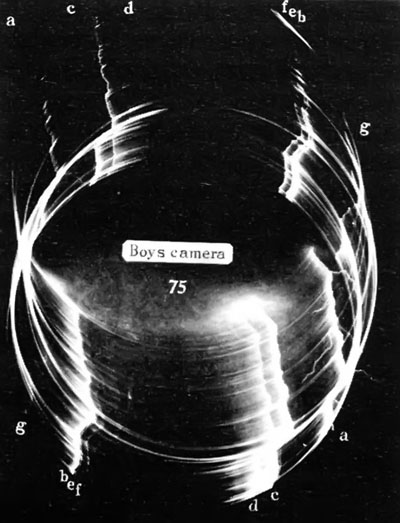
\includegraphics[width=0.6\linewidth]{fyz_fig702.jpg}
      \caption{Fotografie blesku získaná kamerou „Boys“ [Schonland, Malan a Colens, Proc. Roy. Soc.,
               London, Vol. 152 (1935)] (\cite[s.~707]{Feynman02})}
      \label{fyz:fig702}
    \end{figure}

    Nyní popíšeme vlastní blesk. To, jak probíhá, se přesně neví. Zde uvedeme kvalitativní popis
    toho, jak se blesk jeví, ale obejdeme příčiny, proč by měl blesk probíhat tak, jak se zdá, že
    probíhá. Budeme uvažovat pouze obvyklý případ oblaku se zápornou částí nad rovinatou krajinou.
    Oblak má záporný potenciál vzhledem k zemskému povrchu pod sebou, takže záporné elektrony jsou
    urychlovány k zemi. Dochází k následujícím jevům. Vše začíná tím, co se nazývá stupňovitý vůdčí
    výboj (též „lídr“), který není tak oslňující jako vlastní úder blesku. Na fotografiích můžeme na
    začátku vidět malou jasnou skvrnu, která se velkou rychlostí (šestina rychlosti světla!)
    pohybuje dolů. Projde pouze zhruba 50 m a zastaví se. Stojí asi \SI{50}{\us} a potom provede
    další krok. Znovu se zastaví a projde další úsek atd. K zemi se pohybuje sledem kroků po dráze,
    která vypadá tak, jak ukazuje obr. \ref{fyz:fig703}. Ve vůdčím výboji jsou záporné náboje z
    oblaku; celý kanál je plný záporného náboje.


    \begin{figure}[ht!] %\ref{fyz:fig703}
      \centering
      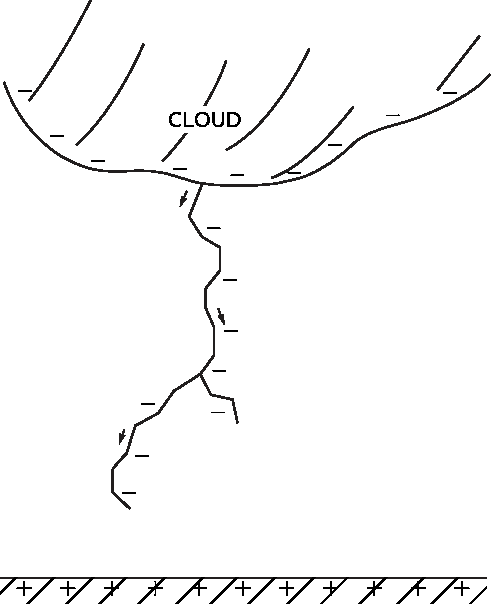
\includegraphics[width=0.6\linewidth]{fyz_fig703.pdf}
      \caption{Vznik vůdčího výboje (\cite[s.~707]{Feynman02})}
      \label{fyz:fig703}
    \end{figure}

    Kromě toho rychlým pohybem nábojů, jenž vůdčí výboj vyvolává, se vzduch ionizuje a podél jeho
    dráhy se stává vodivým. V okamžiku, kdy se vůdčí výboj dotkne zemského povrchu, vzniká vodivý
    „drát“, který sahá až k oblaku a je vyplněn záporným nábojem. Teď konečně může záporný náboj z
    oblaku prostě vytéct Jako první to udělají elektrony ze spodní části vůdčího výboje; vyhrnou se
    dolů a zanechávají za sebou kladný náboj. Ten přitahuje další záporné náboje z vyšších oblastí
    vůdčího výboje, které se postupně vyroní atd. Vytvořeným kanálem nakonec vyteče velkou rychlostí
    všechen záporný náboj z nějaké části oblaku. Ten úder blesku, který vidíme, se proto šíří od
    země nahoru jak je to vyznačeno na obr. \ref{fyz:fig704}. Tento hlavní úder - zdaleka
    nejjasnější část úkazu - se opravdu nazývá \emph{zpětný úder}. Vydává velmi jasné světlo a
    teplo, které způsobí prudkou expanzi vzduchu vyvolávající zadunění hromu.

    Proud v úderu blesku dosahuje v maximu až 10 000 ampérů a unáší dolů zhruba 20 coulombů. Ale
    ještě nejsme na konci. Po uplynutí snad několika setin sekundy od vyhasnutí zpětného výboje
    přichází dolů další úder. Ale nyní už nedělá žádné pauzy. Nazývá se temný vůdčí výboj a celou
    cestu shora dolů projde naráz. Plnou parou se žene po staré trase, protože je tam dostatek
    trosek, které pro něj vytvářejí nejschůdnější cestu. Nový lídr je opět naplněn záporným nábojem.
    Ve chvíli, kdy se dotkne zemského povrchu - bác! - objevuje se zpětný úder, řítící se po téže
    dráze vzhůru. My uvidíme blesk ještě jednou a ještě jednou a ještě jednou. Někdy přeskočí jednou
    nebo dvakrát, někdy pět nebo desetkrát. Bylo zaznamenáno až 42 přeskoků po téže dráze, ale vždy
    za sebou v rychlém sledu.

    \begin{figure}[ht!] %\ref{fyz:fig704}
      \centering
      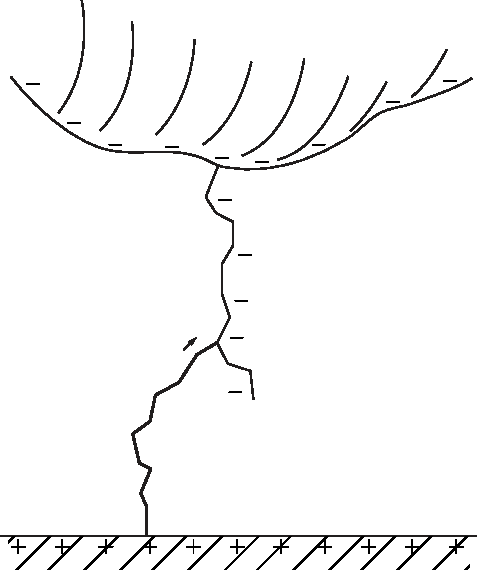
\includegraphics[width=0.6\linewidth]{fyz_fig704.pdf}
      \caption{Při blesku se zpětný úder řítí vzhůru po dráze vytvořené vůdčím výbojem
               (\cite[s.~707]{Feynman02})}
      \label{fyz:fig704}
    \end{figure}

    Jindy se situace ještě více zkomplikuje. Například po jedné ze svých zastávek se může vůdčí
    výboj rozvětvit vysláním dvou odnoží, obou k zemi, ale v trochu odlišných směrech, jak ukazuje
    obr. \ref{fyz:fig703}. Co se stane potom, závisí na tom, zda jedna větev dosáhne zemského
    povrchu výrazně dříve než druhá. Stane-li se tak, jasný zpětný úder (záporného náboje vrhaného
    do země) si udělá cestu vzhůru po té větvi, jež se dotýká země, a když na cestě k oblaku dosáhne
    a míjí bod větvení, objevuje se jasný výboj směrem dolů po druhé větvi. Proč? Protože z oblaku
    se vyhrne záporný náboj, a to je to, co rozsvěcuje blesk. Tento náboj se při vrcholu sekundární
    větve uvede do pohybu, postupně vyprazdňuje následující, delší úseky větve, takže se objevuje
    jasný záblesk směřující po této větvi dolů a zároveň proniká i nahoru do oblaku. Stane-li se
    však, že jedna z těchto přídavných větví vůdčího výboje dosáhne povrchu téměř současně s
    původním vůdčím výbojem, může někdy dojít k tomu, že temný úder druhého blesku půjde po druhé
    větvi. Potom uvidíte první hlavní záblesk na jednom místě a druhý na jiném místě. Jde o variantu
    původní představy.

    Kromě toho je náš popis pro oblast velmi blízko u země zjednodušený. Existují důkazy, že když se
    stupňovitý vůdčí výboj dostane do výšky asi \SI{100}{\m} od země, zvedá se k němu z povrchu Země
    protisměrný výboj. Pole pravděpodobně nabývá velikosti postačující pro vznik korónového výboje.
    Je-li tam ostrý objekt, například budova s hrotem navrchu, a prochází-li dolů vůdčí výboj, pole
    se natolik zvětší, že z ostrého výčnělku vyrazí samostatný výboj a spojí se s vůdčím výbojem.
    Blesk má sklon udeřit do takového hrotu.